\documentclass[11pt,compress,t,notes=noshow, xcolor=table]{beamer}
\usepackage[]{graphicx}\usepackage[]{color}
% maxwidth is the original width if it is less than linewidth
% otherwise use linewidth (to make sure the graphics do not exceed the margin)
\makeatletter
\def\maxwidth{ %
  \ifdim\Gin@nat@width>\linewidth
    \linewidth
  \else
    \Gin@nat@width
  \fi
}
\makeatother

\definecolor{fgcolor}{rgb}{0.345, 0.345, 0.345}
\newcommand{\hlnum}[1]{\textcolor[rgb]{0.686,0.059,0.569}{#1}}%
\newcommand{\hlstr}[1]{\textcolor[rgb]{0.192,0.494,0.8}{#1}}%
\newcommand{\hlcom}[1]{\textcolor[rgb]{0.678,0.584,0.686}{\textit{#1}}}%
\newcommand{\hlopt}[1]{\textcolor[rgb]{0,0,0}{#1}}%
\newcommand{\hlstd}[1]{\textcolor[rgb]{0.345,0.345,0.345}{#1}}%
\newcommand{\hlkwa}[1]{\textcolor[rgb]{0.161,0.373,0.58}{\textbf{#1}}}%
\newcommand{\hlkwb}[1]{\textcolor[rgb]{0.69,0.353,0.396}{#1}}%
\newcommand{\hlkwc}[1]{\textcolor[rgb]{0.333,0.667,0.333}{#1}}%
\newcommand{\hlkwd}[1]{\textcolor[rgb]{0.737,0.353,0.396}{\textbf{#1}}}%
\let\hlipl\hlkwb

\usepackage{framed}
\makeatletter
\newenvironment{kframe}{%
 \def\at@end@of@kframe{}%
 \ifinner\ifhmode%
  \def\at@end@of@kframe{\end{minipage}}%
  \begin{minipage}{\columnwidth}%
 \fi\fi%
 \def\FrameCommand##1{\hskip\@totalleftmargin \hskip-\fboxsep
 \colorbox{shadecolor}{##1}\hskip-\fboxsep
     % There is no \\@totalrightmargin, so:
     \hskip-\linewidth \hskip-\@totalleftmargin \hskip\columnwidth}%
 \MakeFramed {\advance\hsize-\width
   \@totalleftmargin\z@ \linewidth\hsize
   \@setminipage}}%
 {\par\unskip\endMakeFramed%
 \at@end@of@kframe}
\makeatother

\definecolor{shadecolor}{rgb}{.97, .97, .97}
\definecolor{messagecolor}{rgb}{0, 0, 0}
\definecolor{warningcolor}{rgb}{1, 0, 1}
\definecolor{errorcolor}{rgb}{1, 0, 0}
\newenvironment{knitrout}{}{} % an empty environment to be redefined in TeX

\usepackage{alltt}
\newcommand{\SweaveOpts}[1]{}  % do not interfere with LaTeX
\newcommand{\SweaveInput}[1]{} % because they are not real TeX commands
\newcommand{\Sexpr}[1]{}       % will only be parsed by R
\newcommand{\xmark}{\ding{55}}%


\usepackage[english]{babel}
\usepackage[utf8]{inputenc}

\usepackage{dsfont}
\usepackage{verbatim}
\usepackage{amsmath}
\usepackage{amsfonts}
\usepackage{amssymb}
\usepackage{bm}
\usepackage{csquotes}
\usepackage{multirow}
\usepackage{longtable}
\usepackage{booktabs}
\usepackage{enumerate}
\usepackage[absolute,overlay]{textpos}
\usepackage{psfrag}
\usepackage{algorithm}
\usepackage{algpseudocode}
\usepackage{eqnarray}
\usepackage{arydshln}
\usepackage{tabularx}
\usepackage{placeins}
\usepackage{tikz}
\usepackage{setspace}
\usepackage{colortbl}
\usepackage{mathtools}
\usepackage{wrapfig}
\usepackage{bm}
\usepackage{amsmath}
\usepackage{pifont}
\usepackage{xcolor} %colored math symbols

\usetikzlibrary{shapes,arrows,automata,positioning,calc,chains,trees, shadows}
\tikzset{
  %Define standard arrow tip
  >=stealth',
  %Define style for boxes
  punkt/.style={
    rectangle,
    rounded corners,
    draw=black, very thick,
    text width=6.5em,
    minimum height=2em,
    text centered},
  % Define arrow style
  pil/.style={
    ->,
    thick,
    shorten <=2pt,
    shorten >=2pt,}
}

\usepackage{subfig}

% Defines macros and environments
\usepackage{../../style/lmu-lecture}


\let\code=\texttt
\let\proglang=\textsf

\setkeys{Gin}{width=0.9\textwidth}

\setbeamertemplate{frametitle}{\expandafter\uppercase\expandafter\insertframetitle}

\usepackage{bbm}
% basic latex stuff
\newcommand{\pkg}[1]{{\fontseries{b}\selectfont #1}} %fontstyle for R packages
\newcommand{\lz}{\vspace{0.5cm}} %vertical space
\newcommand{\dlz}{\vspace{1cm}} %double vertical space
\newcommand{\oneliner}[1] % Oneliner for important statements
{\begin{block}{}\begin{center}\begin{Large}#1\end{Large}\end{center}\end{block}}


%new environments
\newenvironment{vbframe}  %frame with breaks and verbatim
{
 \begin{frame}[containsverbatim,allowframebreaks]
}
{
\end{frame}
}

\newenvironment{vframe}  %frame with verbatim without breaks (to avoid numbering one slided frames)
{
 \begin{frame}[containsverbatim]
}
{
\end{frame}
}

\newenvironment{blocki}[1]   % itemize block
{
 \begin{block}{#1}\begin{itemize}
}
{
\end{itemize}\end{block}
}

\newenvironment{fragileframe}[2]{  %fragile frame with framebreaks
\begin{frame}[allowframebreaks, fragile, environment = fragileframe]
\frametitle{#1}
#2}
{\end{frame}}


\newcommand{\myframe}[2]{  %short for frame with framebreaks
\begin{frame}[allowframebreaks]
\frametitle{#1}
#2
\end{frame}}

\newcommand{\remark}[1]{
  \textbf{Remark:} #1
}


\newenvironment{deleteframe}
{
\begingroup
\usebackgroundtemplate{
\includegraphics[width=\paperwidth,height=\paperheight]{../style/color/red.png}}
 \begin{frame}
}
{
\end{frame}
\endgroup
}
\newenvironment{simplifyframe}
{
\begingroup
\usebackgroundtemplate{
\includegraphics[width=\paperwidth,height=\paperheight]{../style/color/yellow.png}}
 \begin{frame}
}
{
\end{frame}
\endgroup
}\newenvironment{draftframe}
{
\begingroup
\usebackgroundtemplate{
\includegraphics[width=\paperwidth,height=\paperheight]{../style/color/green.jpg}}
 \begin{frame}
}
{
\end{frame}
\endgroup
}
% https://tex.stackexchange.com/a/261480: textcolor that works in mathmode
\makeatletter
\renewcommand*{\@textcolor}[3]{%
  \protect\leavevmode
  \begingroup
    \color#1{#2}#3%
  \endgroup
}
\makeatother


\input{../../latex-math/basic-math}
\input{../../latex-math/basic-ml}
\input{../../latex-math/ml-nn}

\newcommand{\titlefigure}{figure/backprop_gg_new.png}
\newcommand{\learninggoals}{
  \item Efficiency of backpropagation
  \item Caching
  \item Backpropagation formalism
}

\title{Deep Learning}
\date{}

\begin{document}

\lecturechapter{Basic Backpropagation 2}
\lecture{I2DL}
%%%%%%%%%%%%%%%%%%%%%%%%%%%%%%%%%%%%%%%%%%%%%%%%%%%%%%%%%%%%%%%%%%


\begin{frame} {Backward Computation and Caching}
    In the XOR example, we computed:
    $$\frac{\partial \Lxy}{\partial W_{11}} = 
        \frac{\partial \Lxy}{\partial f_{out}} \cdot  \textcolor{black}{\frac{\partial f_{out}}{\partial f_{in}}} \cdot  \textcolor{black}{\frac{\partial f_{in}}{\partial z_{1,out}}} \cdot  \textcolor{black}{\frac{\partial z_{1,out}}{\partial z_{1,in}}} \cdot  \textcolor{black}{\frac{\partial z_{1,in}}{\partial W_{11}}} $$
  \begin{figure}
    \centering
      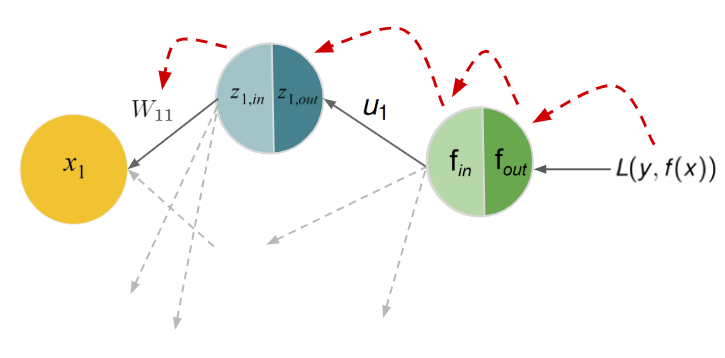
\includegraphics[width=9cm]{figure/backprop_gg1_new.png}
      \caption{All five terms of our chain rule}
  \end{figure}
\end{frame}
%%%%%%%%%%%%%%%%%%%%%%%%%%%%%%%%%%%%%%%%%%%%%%%%%%%%%%%%%%%%%%%%%%

\begin{frame} {Backward Computation and Caching}
Next, let us compute:
      $$\frac{\partial \Lxy}{\partial W_{21}} = 
\frac{\partial \Lxy}{\partial f_{out}} \cdot  \textcolor{black}{\frac{\partial f_{out}}{\partial f_{in}}} \cdot  \textcolor{black}{\frac{\partial f_{in}}{\partial z_{1,out}}} \cdot  \textcolor{black}{\frac{\partial z_{1,out}}{\partial z_{1,in}}} \cdot  \textcolor{black}{\frac{\partial z_{1,in}}{\partial W_{21}}}$$
        \begin{figure}
    \centering
      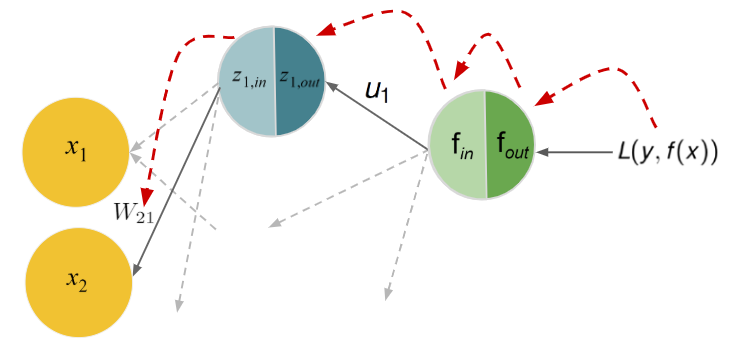
\includegraphics[width=9cm]{figure/backprop_gg_new.png}
      \caption{All five terms of our chain rule}
  \end{figure}
\end{frame}
%%%%%%%%%%%%%%%%%%%%%%%%%%%%%%%%%%%%%%%%%%%%%%%%%%%%%%%%%%%%%%%%%%

\begin{frame} {Backward Computation and Caching}
\begin{itemize}
\item Examining the two expressions:
$$\frac{\partial \Lxy}{\partial W_{11}} = 
\textcolor{violet}{\frac{\partial \Lxy}{\partial f_{out}}} \cdot  \textcolor{violet}{\frac{\partial f_{out}}{\partial f_{in}}} \cdot  \textcolor{violet}{\frac{\partial f_{in}}{\partial z_{1,out}}} \cdot  \textcolor{violet}{\frac{\partial z_{1,out}}{\partial z_{1,in}}} \cdot  \textcolor{black}{\frac{\partial z_{1,in}}{\partial W_{11}}}$$

$$\frac{\partial \Lxy}{\partial W_{21}} =     
\textcolor{violet}{\frac{\partial \Lxy}{\partial f_{out}}} \cdot  \textcolor{violet}{\frac{\partial f_{out}}{\partial f_{in}}} \cdot  \textcolor{violet}{\frac{\partial f_{in}}{\partial z_{1,out}}} \cdot  \textcolor{violet}{\frac{\partial z_{1,out}}{\partial z_{1,in}}} \cdot  \textcolor{black}{\frac{\partial z_{1,in}}{\partial W_{21}}}$$

\item We see that there is significant overlap / redundancy in the two expressions. A huge chunk of the second expression has already been computed while computing the first one.
\item \textbf{Again}: Simply cache these subexpressions instead of recomputing them each time.
\end{itemize}
\end{frame}
%%%%%%%%%%%%%%%%%%%%%%%%%%%%%%%%%%%%%%%%%%%%%%%%%%%%%%%%%%%%%%%%%%

\begin{frame} {Backward Computation and Caching}
\begin{itemize}
\item Let {\small $$\textcolor{violet}{\delta_1}  = \textcolor{violet}{\frac{\partial \Lxy}{\partial z_{1,in}}} = 
\textcolor{violet}{\frac{\partial \Lxy}{\partial f_{out}}} \cdot  \textcolor{violet}{\frac{\partial f_{out}}{\partial f_{in}}} \cdot  \textcolor{violet}{\frac{\partial f_{in}}{\partial z_{1,out}}} \cdot  \textcolor{violet}{\frac{\partial z_{1,out}}{\partial z_{1,in}}}$$} be cached. $\delta_1$ can also be seen as an \textbf{error signal} that represents how much the loss $L$ changes when the input $z_{1,in}$ changes.

\item The two expressions of the previous slide now become,
{\small $$\frac{\partial \Lxy}{\partial W_{11}} = \textcolor{violet}{\delta_1} \cdot \frac{\partial z_{1,in}}{\partial W_{11}} \mbox{ \hspace{0.5cm} \small{and} \hspace{0.5cm}} \frac{\partial \Lxy}{\partial W_{21}} = \textcolor{violet}{\delta_1} \cdot \frac{\partial z_{1,in}}{\partial W_{21}} $$}
where $\delta_1$ is simply "plugged in".
\item As you can imagine, caching subexpressions in this way and plugging in where needed can result in \textbf{massive} gains in efficiency for deep and "wide" neural networks. 
\item In fact, this simple algorithm, which was first applied to neural networks way back in 1985, is \textbf{still} the biggest breakthrough in deep learning.
\end{itemize}
\end{frame}
%%%%%%%%%%%%%%%%%%%%%%%%%%%%%%%%%%%%%%%%%%%%%%%%%%%%%%%%%%%%%%%%%%

\begin{frame} {Backward Computation and Caching}
  \begin{itemize}
    \item On the other hand, if we had done a \textbf{forward} caching of the derivatives
    {\small $$\frac{\partial \Lxy}{\partial W_{11}} = \Bigg(\Bigg(\Bigg( \frac{\partial z_{1,in}}{\partial W_{11}} \frac{\partial z_{1,out}}{\partial z_{1,in}} \Bigg)  \frac{\partial f_{in}}{\partial z_{1,out}} \Bigg) \frac{\partial f_{out}}{\partial f_{in}} \Bigg) \frac{\partial \Lxy}{\partial f_{out}}$$}
      {\small $$\frac{\partial \Lxy}{\partial W_{21}} = 
        \Bigg(\Bigg(\Bigg( \frac{\partial z_{1,in}}{\partial W_{21}} \frac{\partial z_{1,out}}{\partial z_{1,in}} \Bigg)  \frac{\partial f_{in}}{\partial z_{1,out}} \Bigg) \frac{\partial f_{out}}{\partial f_{in}} \Bigg) \frac{\partial \Lxy}{\partial f_{out}}$$}
      there would be no common subexpressions to plug in. We would have to compute the \text{entire} expression for each and every weight!
    \item This would make the computations too inefficient to make gradient descent tractable for large neural networks.
  \end{itemize}
\end{frame}
%%%%%%%%%%%%%%%%%%%%%%%%%%%%%%%%%%%%%%%%%%%%%%%%%%%%%%%%%%%%%%%%%%



\begin{frame} {Backpropagation: Formalism}
  \begin{itemize}
    \item \small{Let us now derive a general formulation of backpropagation.}
    \item \small{The neurons in layers $i-1$, $i$ and $i+1$ are indexed by $j$, $k$ and $m$, respectively.
    \item The output layer will be referred to as layer O.}
   \begin{figure}
    \centering
      \scalebox{1}{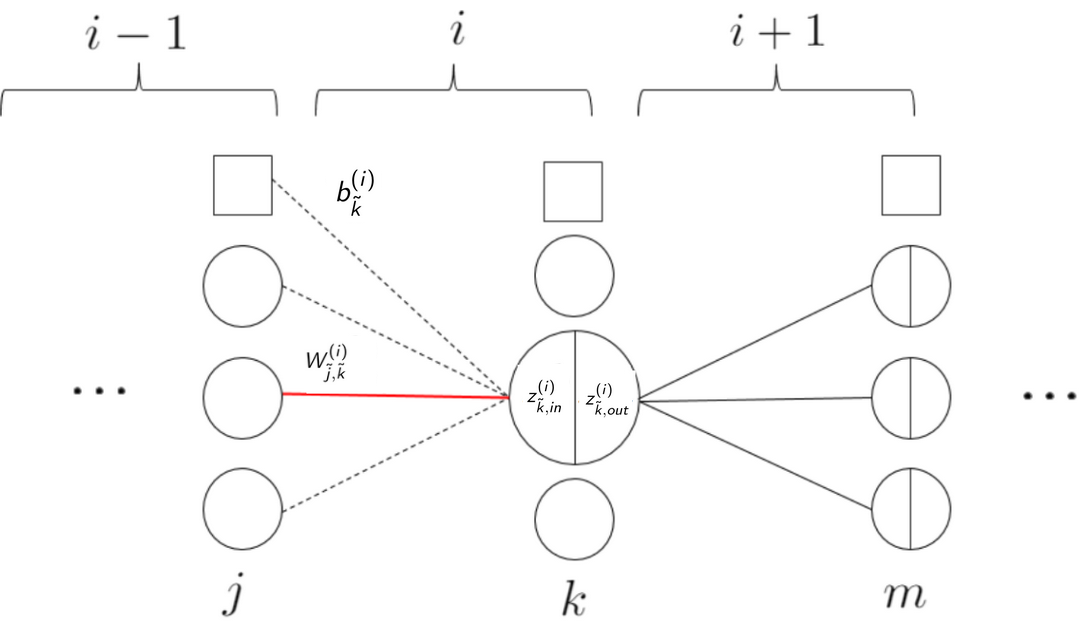
\includegraphics{figure/backnet.png}}
      \tiny{\\Credit: Erik Hallstr\"{o}m}
    \end{figure}
  \end{itemize}
\end{frame}
%%%%%%%%%%%%%%%%%%%%%%%%%%%%%%%%%%%%%%%%%%%%%%%%%%%%%%%%%%%%%%%%%%

\begin{vbframe} {Backpropagation: Formalism}

  \vspace*{-0.3cm}

 \begin{figure}
  \centering
    \scalebox{0.6}{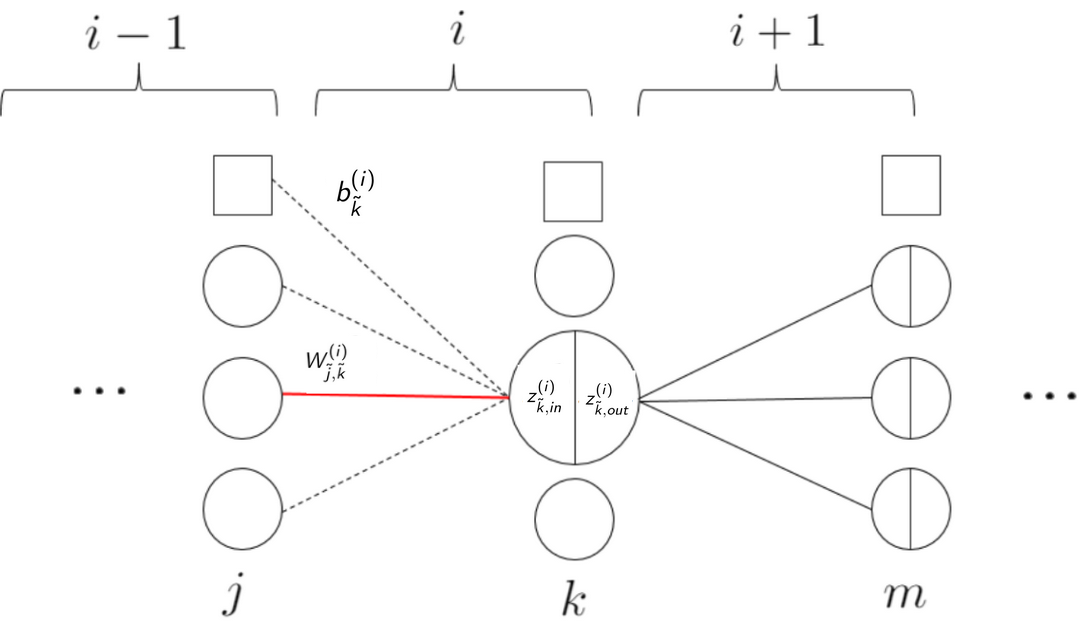
\includegraphics{figure/backnet.png}}
  \end{figure}
  \vspace*{-0.5cm}
  \begin{small}
  \begin{itemize}
    \item Let $\delta_{\tilde{k}}^{(i)}$ (also: error signal) for a neuron $\tilde{k}$ in layer $i$ represent how much the loss $L$ changes when the input $z_{\tilde{k},in}^{(i)}$   changes:
    {\small
      $$\delta_{\tilde{k}}^{(i)} = \frac{\partial L}{\partial z_{\tilde{k},in}^{(i)}} =  \frac{\partial L}{\partial z_{\tilde{k},out}^{(i)}} \frac{\partial z_{\tilde{k},out}^{(i)}}{\partial z_{\tilde{k},in}^{(i)}}   =  \sum_m \Bigg( \frac{\partial L}{\partial z_{m,in}^{(i+1)}} \frac{\partial z_{m,in}^{(i+1)}}{\partial z_{\tilde{k},out}^{(i)}} \Bigg) \frac{\partial z_{\tilde{k},out}^{(i)}}{\partial z_{\tilde{k},in}^{(i)}} $$}

    \item Note: The sum in the expression above is over all the neurons in layer $i+1$. This is simply an application of the (multivariable) chain rule.
  \end{itemize}
  \end{small}
\end{vbframe}
%%%%%%%%%%%%%%%%%%%%%%%%%%%%%%%%%%%%%%%%%%%%%%%%%%%%%%%%%%%%%%%%%%

\begin{frame} {Backpropagation: Formalism}
 Using 
 \vspace*{-5mm}
        {\footnotesize \begin{eqnarray*}
          \textcolor{blue}{z_{\tilde{k},out}^{(i)}} &=& \textcolor{blue}{\sigma(z_{\tilde{k},in}^{(i)})} \\
          \textcolor{violet}{z_{m,in}^{(i+1)}} &=& \textcolor{violet}{\sum_k W_{k,m}^{(i+1)}z_{k,out}^{(i)} + b_m^{(i+1)}}
        \end{eqnarray*}}
we get: 
      \vspace{-0.2cm}
      {\footnotesize \begin{eqnarray*}
      \delta_{\tilde{k}}^{(i)} &=& \sum_m \Bigg( \frac{\partial L}{\partial z_{m,in}^{(i+1)}} \frac{\partial \textcolor{violet}{z_{m,in}^{(i+1)}}}{\partial z_{\tilde{k},out}^{(i)}} \Bigg) \frac{\partial \textcolor{blue}{z_{\tilde{k},out}^{(i)}}}{\partial z_{\tilde{k},in}^{(i)}}  \\
       &=& \sum_m \Bigg( \frac{\partial L}{\partial z_{m,in}^{(i+1)}} \frac{\partial \left(\textcolor{violet}{\sum_k W_{k,m}^{(i+1)}z_{k,out}^{(i)} + b_m^{(i+1)}}\right)}{\partial z_{\tilde{k},out}^{(i)}} \Bigg) \frac{\partial \textcolor{blue}{\sigma(z_{\tilde{k},in}^{(i)})}}{\partial z_{\tilde{k},in}^{(i)}}  \\
      &=& \sum_m \Bigg( \frac{\partial L}{\partial z_{m,in}^{(i+1)}} \textcolor{violet}{W_{\tilde{k},m}^{(i+1)}} \Bigg) \textcolor{blue}{\sigma'(z_{\tilde{k},in}^{(i)})} = \sum_m \Bigg(  \delta_{\tilde{k}}^{(i+1)} \textcolor{violet}{W_{\tilde{k},m}^{(i+1)}} \Bigg) \textcolor{blue}{\sigma'(z_{\tilde{k},in}^{(i)})} 
      \end{eqnarray*}}\\
      Therefore, we now have a \textbf{recursive definition} for the error signal of a neuron in layer $i$ in terms of the error signals of the neurons in layer $i+1$ and, by extension, layers \{i+2, i+3 \ldots , O\}!
\end{frame}
%%%%%%%%%%%%%%%%%%%%%%%%%%%%%%%%%%%%%%%%%%%%%%%%%%%%%%%%%%%%%%%%%%

\begin{frame} {Backpropagation: Formalism}
  \begin{itemize}
    \item Given the error signal $\delta_{\tilde{k}}^{(i)}$ of neuron $\tilde{k}$ in layer $i$, the derivative of loss $L$ w.r.t. to the weight $W_{\tilde{j},\tilde{k}}$ is simply:
        $$
           \frac{\partial L}{\partial W_{\tilde{j},\tilde{k}}^{(i)}} = \frac{\partial L}{\partial z_{\tilde{k},in}^{(i)}} \frac{\partial z_{\tilde{k},in}^{(i)}}{\partial W_{\tilde{j},\tilde{k}}^{(i)}} 
           = \delta_{\tilde{k}}^{(i)} z_{\tilde{j},out}^{(i-1)} $$
        because $z_{\tilde{k},in}^{(i)} = \sum_j W_{j,\tilde{k}}^{(i)}z_{j,out}^{(i-1)}  + b_{\tilde{k}}^{(i)}$
    \item Similarly, the derivative of loss $L$ w.r.t. bias $b_{\tilde{k}}^{(i)}$ is:
      $$ \frac{\partial L}{\partial b_{\tilde{k}}^{(i)}} = \frac{\partial L}{\partial z_{\tilde{k},in}^{(i)}} \frac{\partial z_{\tilde{k},in}^{(i)}}{\partial b_{\tilde{k}}^{(i)}} = \delta_{\tilde{k}}^{(i)}$$
  \end{itemize}
\end{frame}
%%%%%%%%%%%%%%%%%%%%%%%%%%%%%%%%%%%%%%%%%%%%%%%%%%%%%%%%%%%%%%%%%%

\begin{frame} {Backpropagation: Formalism}
\begin{itemize}
\item We have seen how to compute the error signals for individual neurons. It can be shown that the error signal $\bm{\delta}^{i}$ for an entire layer $i$ can be computed as follows ($\odot$ = element-wise product):
\begin{itemize}
\item $\bm{\delta}^{(O)} = \nabla_{f_{out}}L \odot \tau'(f_{in})$
\item $\bm{\delta}^{(i)} = W^{(i+1)}\bm{\delta}^{(i+1)} \odot \sigma'(z_{in}^{(i)})$
\end{itemize}
\item As we have seen earlier, the error signal for a given layer $i$ depends recursively on the error signals of \textbf{later} layers \{i+1, i+2, \ldots , O\}.
\item Therefore, backpropagation works by computing and storing the error signals \textbf{backwards}. That is, starting at the output layer and ending at the first hidden layer. This way, the error signals of later layers \textbf{propagate backwards} to the earlier layers.
\item The derivative of the loss $L$ w.r.t. a given weight is computed efficiently by plugging in the cached error signals thereby avoiding expensive and redundant computations. 
\end{itemize}
\end{frame}
%%%%%%%%%%%%%%%%%%%%%%%%%%%%%%%%%%%%%%%%%%%%%%%%%%%%%%%%%%%%%%%%%%

\endlecture
\end{document}